\documentclass{article}

\usepackage{verbatim}				% For using a text file verbatim, e.g. for code
\usepackage{graphicx}				% For adding images
\graphicspath{{images/}}		% Specify image directory path
\usepackage{amsmath}				% For math
\usepackage{mathtools}
\usepackage{bm}					% For bold math symbols
\usepackage{cancel}					% For math cancellation
\usepackage{lipsum}
\usepackage{mwe}
%\usepackage{centernot}				% For negating any symbol
\usepackage{amssymb}				% For extra symbols
\usepackage[colorlinks = true,
		     linkcolor = blue,
		     urlcolor = blue,
		     citecolor = blue,
		     anchorcolor = blue]{hyperref}				% For hyperlinks
\usepackage{color}				% For colored text
%\usepackage{multido}				% For loops \multido{<vars>}{<repetitions>}{<stuff to repeat>}
\usepackage{braket}				% For braket notation
%\usepackage{physics}				% Lots of goodies
%\usepackage[margin=1in]{geometry}	% For adjusting the margin size

% Raise the title a bit
\usepackage{titling}
\setlength{\droptitle}{-10em}

\title{%
	Equilibrium Phases in the 1-D Hubbard Model \\
	\large PHYS 416}
\author{Johann Gan}
\date{April 11, 2019}


% Custom operators - requires amsmath package
%\DeclareMathOperator*{\argmin}{arg\,min}
%\DeclareMathOperator*{\argmax}{arg\,max}

% Custom commands
\newcommand{\p}{\newline\newline}		% Double newline (paragraph without indent)
\newcommand{\eval}{\bigg\rvert} 		% Evaluation with bounds bar
\newcommand{\lagr}{\mathcal{L}}		% Lagrangian
\newcommand{\bmhat}[1]{
	\hat{\bm{#1}}
}
\newcommand{\chk}{\>\>\checkmark}
\newcommand{\bigo}{\mathcal{O}}
\newcommand{\dt}{\Delta t}
\newcommand{\parder}[3][1]{
	\ifnum1=#1\relax
		\frac{\partial #2}{\partial #3}
	\else
		\frac{\partial^#1 #2}{\partial #3^#1}
	\fi
}
\newcommand{\D}[2]{
\ifnum1=#2\relax
		\frac{\partial}{\partial #1}
	\else
		\frac{\partial^#2}{\partial #1^#2}
	\fi
}
\newcommand{\pvec}[1]{\vec{#1}\mkern2mu\vphantom{#1}'} 	% Primed vector
%\newcommand{\innerfencepost}[3]{
%	\multido{\i=1+1}{\number\numexpr#1-1\relax}{#2#3}#2
%}
%\newcommand{\outerfencepost}[3]{
%	\multido{\i=1+1}{#1}{#3#2}#3
%}
\newcommand{\nicegraphic}[2][1]{
	\begin{center}
		\includegraphics[width=#1\textwidth]{#2}
	\end{center}
}


\begin{document}

\maketitle
% Separate title page
%\pagenumbering{gobble}				% The title page isn't page "1"
%\newpage
%\pagenumbering{arabic}

\section{Background}
The Hubbard model is one of the simplest models of interacting fermions in a lattice, and has been an important tool in studying many-body quantum physics. Understanding states of matter where quantum interactions dominate behavior is key for designing useful materials with new and exotic properties. While crude, the Hubbard Hamiltonian nevertheless exhibits such quantum interactions, and many physicists believe the model contains the essential physics governing high-temperature superconductivity in cuprates. More recently, the advent of ultracold atomic systems has enabled experimental realization of the Hubbard Hamiltonian, sparking renewed interest in the model.

Studying the Hubbard model, as with most many-body quantum systems, poses severe computational challenges. The number of variables grows exponentially with system size (as opposed to linearly in the classical case) due to quantum superposition, limiting even state-of-the-art direct simulation to around only 50 particles. Even after extensive study, the Hubbard model has not been completely solved in dimensions above 1.

\section{This Project}
To keep things simple, I chose to investigate the 1-D Hubbard model with spin-1/2 fermions (e.g. electrons). My central question was: How do global, steady-state properties like magnetization and conductivity change when interactions (e.g. Coulomb repulsion) are allowed between fermions? What is the dependence on the strength of these interactions, and does this change with the density of the system?

More precisely, the Hubbard Hamiltonian is,

\begin{align*}
\hat H = -t\sum_{i\sigma}\left(\hat c_{i\sigma}^\dag\hat c_{(i+1)\sigma} + \hat c_{(i+1)\sigma}^\dag\hat c_{i\sigma}\right) + U\sum_i\hat n_{i\uparrow}\hat n_{i\downarrow} - \mu\sum_i\left(\hat n_{i\uparrow} + \hat n_{i\downarrow}\right)
\end{align*}
The first term lets fermions ``hop'' between neighboring sites with ``hopping amplitude'' $t$. The second term adds a repulsion $U$ between two fermions occupying the same site. The last term controls the total particle number via the chemical potential $\mu$. The precise question then becomes: How do equilibrium properties change under different values of $U/t$ and $\mu$ (or particle density $\rho(\mu)$)?

\section{Methods}
The main equation is the time-independent Schr\"odinger equation,
\begin{align*}
\hat H\Ket{\psi} = E\Ket{\psi}
\end{align*}
which is an eigenvalue problem.

\subsection{Exact Diagonalization} The straightforward approach is exact diagonalization (ED), i.e. setting up the Hamiltonian matrix and numerically solving the eigenvalue problem. Since the Hamiltonian conserves total particle number, it actually suffices to diagonalize constituent subspaces of the full Hamiltonian with fixed particle numbers. The energies are the same, but the problem size is significantly reduced. I used this technique to investigate the band structure (energy levels) of small systems.

\subsection{Mean Field Theory} To analyze large systems, I used mean field theory (MFT). MFT approximates a pairwise interaction between fermions (hard) as a single-particle interaction with a ``mean field'' (easier). This amounts to replacing terms in the Hamiltonian with expectations. These expectations are different depending on whether we assume ferromagnetic order (adjacent spins aligned) or antiferromagnetic order (adjacent spins anti-aligned). It turns out that MFT simplifies both cases enough to derive analytic expressions for the energy levels.

Given analytic energy expressions, I constructed a magnetic phase diagram over different $U/t$ and $\rho$. I iterated over different phase space points, and determined the equilibrium phase by using the analytic energy expressions to see whether ferromagnetism or antiferromagnetism (or paramagnetism - a lack of either) gives a lower energy state.

I also did an MFT calculation of the compressibility, $\parder{\rho}{\mu}$, of the system under different $U/t$. The $\rho(\mu)$ curves are computable using MFT as above, except allowing particle numbers to fluctuate. Since the expectation values are \textit{dependent} on the particle numbers, I used an iterative calculation to continually update $\rho$ until it settled to a self-consistent value. Combining this with multiple trials and randomized initial guesses gave consistent results.

\section{Results and Interpretations}
\subsection{Magnetic Phase Diagram}
The computed phase diagram is shown in Figure \ref{fig:phase}. Figure \ref{fig:magnetism} provides an illustration of different magnetic phases. From the diagram, it is clear that both interaction strength and particle density have some effect on the equilibrium state of the fermions. The symmetry about $\rho = 1$ demonstrates \textit{particle-hole symmetry} of the Hubbard Hamiltonian. Holes appear to move around and interact just like fermions themselves \cite{scalettar}. The diagram makes physical sense if we consider three cases.

\begin{figure}[h]
\nicegraphic[0.9]{fermi_hubbard_phase_diagram}
\caption{Magnetic phase diagram for the 1-D Hubbard chain. The left shows the phase at different points in $U/t-\rho$ phase space. Blue, green, and red denote ferro-, para-, and antiferromagnetism. The right plot shows the magnitude of the relevant magnetization (normal or staggered).}
\label{fig:phase}
\end{figure}

\begin{figure}[h]
\begin{tabular}{ccc}
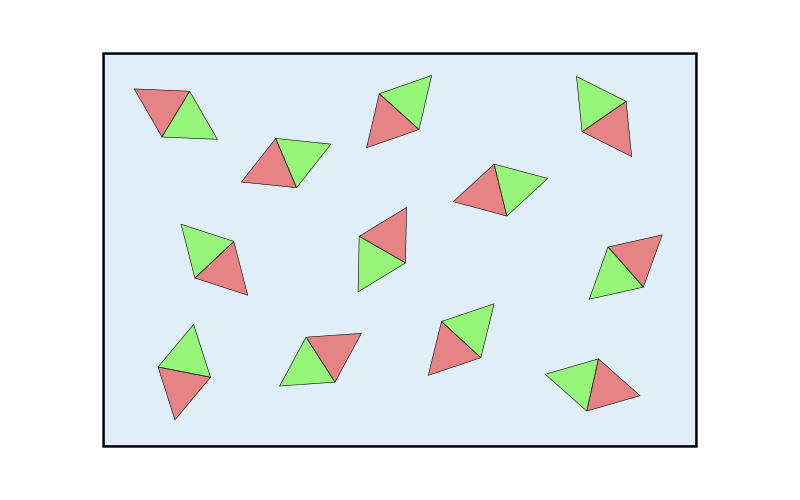
\includegraphics[width=0.32\textwidth,height=5em]{paramagnetism} & 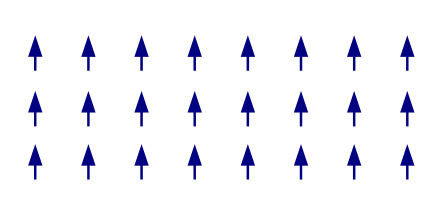
\includegraphics[width=0.32\textwidth]{ferromagnetism} & 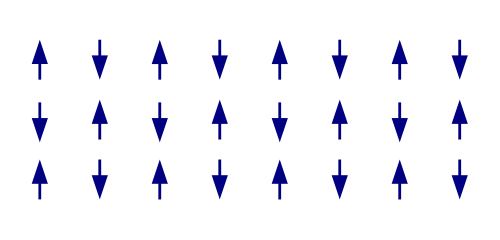
\includegraphics[width=0.32\textwidth]{antiferromagnetism}
\end{tabular}
\caption{Different types of magnetism. Left: paramagnetism, no order. Middle: ferromagnetism, spins aligned. Right: antiferromagnetism, spins anti-aligned. \href{https://commons.wikimedia.org/wiki/File:Ferromagnetic_ordering.svg}{``Ferromagnetic ordering''} and \href{https://commons.wikimedia.org/wiki/File:Antiferromagnetic_ordering.svg}{``Antiferromagnetic ordering''} by \href{https://commons.wikimedia.org/wiki/User:Schmid}{Michael Schmid} are licensed under \href{https://creativecommons.org/licenses/by-sa/3.0/deed.en}{CC BY-SA 3.0}.}
\label{fig:magnetism}
\end{figure}

\paragraph{Case 1: Low interaction, $\bm{\rho}$ away from 1} For low density, we essentially have a dilute gas, and particles move freely without correlating. For high density, the same things applies, just with holes.

\paragraph{Case 2: High interaction $\bm{\rho}$ away from 1} The kinetic energy tends to make the particles spread out through the lattice and delocalize over all sites, encroaching on each other's space. If spins are aligned, the Pauli exclusion principle will help keep the particles apart, thus avoiding the energy cost of Coulomb repulsion. Thus, the spins of fermions tend to align.

\paragraph{Case 3: High/low interaction, $\bm{\rho \sim 1}$} It can be shown that for $\rho = 1$ and high interaction, the Hubbard model maps to the spin-1/2 \textit{Heisenberg model} of interacting spins with $J = 4t^2/U$ \cite{scalettar}. The Heisenberg Hamiltonian is,
\begin{align*}
\hat H = J\sum_i \bm S_i \cdot \bm S_{i+1}
\end{align*}
This model clearly displays antiferromagnetism, since to minimize the energy the dot product should be negative, thus the spins tend to anti-align. If the Hubbard model maps to the Heisenberg model, we should also expect antiferromagnetism for $\rho = 1$ and high interaction, and a small deviation from there shouldn't change the physics too much. It seems that at \textit{exactly} half filling, the antiferromagnetism persists all the way down to weak interactions.

\subsection{Compressibility}
Compressibility represents how easy it is to force extra particles into the system by raising the external chemical potential. What makes it interesting is that it is simpler to compute than conductivity, but it still gives information about the system's ability to conduct, since a system that permits adding new electrons should also be permissive to electron transport.

Figures \ref{fig:compresslow} (low to moderate interactions) and \ref{fig:compresshigh} (high interactions) reveal some interesting physics. With no interactions, density increases smoothly with the chemical potential, as we would expect. When moderate interactions are turned on, there are saturation points at $\rho = 0, 2$ that we didn't see before, but these are just the expected zero and full filling. More interesting is that there is a single antiferromagnetic point at $\mu = 0$, $\rho = 1$, which also corresponds to a slowdown in the filling rate. The high interaction cases bring this trend to its extreme. Around $\mu = 0$ we see a \text{totally flat} region of the $\rho(\mu)$ curve! At half-filling, turning up the external potential doesn't do anything for a while, which makes it an insulator! This demonstrates a so-called ``Mott insulating phase,'' where a material which would be conducting without interactions becomes insulating due to electron-electron interactions. Interestingly, this Mott insulating phase also seems to be related to the onset of antiferromagnetism.

\begin{figure}
\nicegraphic{fermi_hubbard_compressibility_U0_t4}
\nicegraphic{fermi_hubbard_compressibility_U1_t1}
\caption{Compressibility under low or moderate interactions. Top: no interactions, the compressibility is fairly constant. Bottom: moderate interactions, the compressibility bends down near $\mu = 0$, $\rho = 1$ with the minimum happening exactly in an antiferromagnetic phase. The $\rho(\mu)$ curve's ascent is slowed a little at $\mu = 0$.}
\label{fig:compresslow}
\end{figure}
\begin{figure}
\nicegraphic{fermi_hubbard_compressibility_U4_t1}
\nicegraphic{fermi_hubbard_compressibility_U8_t1}
\caption{Compressibility under high interactions. Top: high interactions, there is a clear ``Mott plateau'' around $\mu = 0$ where compressibility (and likely also conductivity!) drops to zero, indicating a Mott insulating phase. The plateau also corresponds with an antiferromagnetic phase. Bottom: highest interactions, similar features to high interactions, just with a larger Mott plateau.}
\label{fig:compresshigh}
\end{figure}

\subsection{Band Structure}
Band structure is another probe of the conductive properties of a material. If the highest-energy electrons at the top of the Fermi sea have lots of easy-to-access excited states (a very small energy gap), these conduction electrons are readily mobile to conduct electricity. On the other hand, if there is a large gap between the Fermi energy and the next excited state, it becomes very hard to excite conduction electrons, and the material becomes insulating.

The band structure of small ($n \leq 7$) Hubbard chains was computed directly using ED under periodic boundary conditions. The band structure for $n = 6$ and $n = 7$ under $U/t = 0$ and $U/t = 100$ are depicted in Figures \ref{fig:band60} through \ref{fig:band7}. Figure \ref{fig:band60} shows the band structure with $n = 6$ and no interactions. The Fermi level is comfortably within a conduction band with many states available for conduction; the system is a conductor. Turning on interactions changes things. Figure \ref{fig:band6100} shows the band structure with $U/t = 100$. The former conduction band has now spread out, leaving far fewer states available for conduction. This is another way to view the Mott insulating transition we saw earlier; electron-electron repulsion opens up an energy gap, which must be overcome before more particles can be added. Figure \ref{fig:band7} tells a similar story, but with $n = 7$. Turning on interactions introduces a very obvious band gap, which drives a conductor-to-Mott-insulator transition.

\begin{figure}
\nicegraphic[0.9]{fermi_hubbard_bands_n6_U0_t1}
\nicegraphic[0.9]{fermi_hubbard_bands_zoomed_n6_U0_t1}
\caption{Bands for $n = 6$, $U/t = 0$. The bottom plot is a zoomed in picture. There are plenty of conduction states at the Fermi level. Note the y-axis scale of $10^{-14}$.}
\label{fig:band60}
\end{figure}
\begin{figure}
\nicegraphic[0.9]{fermi_hubbard_bands_n6_U100_t1}
\nicegraphic[0.9]{fermi_hubbard_bands_zoomed_n6_U100_t1}
\caption{Bands for $n = 6$, $U/t = 100$. The bottom plot is a zoomed in picture. The conduction band has split, making it harder to excite many conduction electrons. Note the y-axis scale is now of order 1.}
\label{fig:band6100}
\end{figure}
\begin{figure}
\nicegraphic[0.9]{fermi_hubbard_bands_n7_U0_t1}
\nicegraphic[0.9]{fermi_hubbard_bands_n7_U100_t1}
\caption{Bands for $n = 7$, $U/t = 0, 100$. Top: $U/t = 0$, there are tons of conduction states at the Fermi level. Bottom: $U/t = 100$, a clear band gap has opened up at the Fermi level due to electron-electron repulsion.}
\label{fig:band7}
\end{figure}

\section{Conclusion}
Using MFT and ED, I investigated magnetism and conductivity in the Hubbard model. It is clear that the introduction of interaction between fermions leads to interesting physics, giving rise to both ferromagnetic and antiferromagnetic order, as well as creating band gaps and Mott insulating phases. Even in 1-D and without thermal fluctuations, the richness of the Hubbard model is quite apparent. This project has only scratched the surface.

\section{Validation}
It is surprisingly hard to find concrete references to compare results to. Scalettar\cite{scalettar} p. 8 shows the Mott plateau similar to those in my compressibility plots, so that is probably correct. The description of the upper and lower Hubbard bands with $n = 2$ sites on p. 17 of Scalettar\cite{scalettar} also matches the physics I observed in my band structure plots. I don't have a reference for my phase diagram, but it makes physical sense, and the fact that it shows particle-hole symmetry and the mapping to the Heisenberg model provides some degree of verification that the physics is correct.

\newpage
\section{Code Documentation}
Code documentation on programs and usage is contained in a separate document. The Python files themselves contain extensive docstrings and comments describing the details of implementation.

\bibliographystyle{abbrv}
\bibliography{biblio}

\end{document}